\subsection{Matching to parton showers with GENEVA}
%\subsection{Matching to parton showers with {\normalfont\scshape GENEVA}} 

%\textit{Authors:} Simone Alioli, Giulia Marinelli, Davide Napoletano (2507.08558)\\

\textbf{Simone Alioli, Giulia Marinelli, Davide Napoletano~\cite{Alioli:2025xcu}.}

\noindent Given the absence of exact results for the three-loop NNLO massive contributions,
to achieve NNLO accuracy we can employ several approximations.
In particular, we can exploit the similarity to the production of a single Higgs boson
in gluon fusion, and apply a reweighting procedure to the unknown virtual matrix
elements using the massive Born ones.
One such approximation is dubbed \ftapprox discussed in the previous section~\cite{Frederix:2014hta,Maltoni:2014eza,Grazzini:2018bsd}, where both the real-virtual and double-virtual contributions
are reweighted to the Born matrix elements.
In the case of real-virtual corrections, this implies that
\begin{equation}
  V_{1}\left(\Phi_1\right) = V_{1}\left(\Phi_1,m_t\to\infty\right)
  \frac{B_1\left(\Phi_1,m_t\right)}
  {B_1\left(\Phi_1,m_t\to\infty\right)}\,,
\end{equation}
where $\Phi_1$ represents the double Higgs boson plus one parton phase space, $V_1,\, B_1$
are the relative virtual and Born contributions, respectively.

The case of the double-virtual contribution is instead slightly more subtle.
In the \geneva framework, we include this contribution through the matching
to the resummation of the slicing variable employed to perform the fixed-order
calculation,
which in turn is used to evaluate the contribution to the cross section
below the resolution variable cut~\cite{Alioli:2012fc}.
For this purpose, we employ the zero-jettiness~\cite{Stewart:2010tn} ($\mathcal{T}_0$) as a resolution variable.
When $\mathcal{T}_0 \muchless Q$ (with $Q$ the hard scale,
chosen here as the Higgs boson pair invariant mass $m_{hh}$), the cross section
factorizes according to Soft Collinear Effective Theory (SCET).
In this regime,
large logarithms of $\mathcal{T}_0/Q$ are resummed systematically up to
next-to-next-to-leading logarithmic primed (NNLL$^\prime$) accuracy.
At leading power in $\mathcal{T}_0^{\mathrm{cut}} / m_{hh}$, we can write the differential cross section
as
\begin{equation}\label{eq:convolutionmess}
  \frac{\mathrm{d} \sigma^{\rm SCET}}{\mathrm{d} \Phi_0 \, \mathrm{d} \mathcal{T}_0} =
  H_{{\scriptscriptstyle gg \to HH }}(Q^2,\mu) \int B_g(t_a,x_a,\mu) \,
  B_g(t_b,x_b,\mu) \, S_{gg}\left( \mathcal{T}_0 - \frac{t_a+t_b}{Q}, \mu \right) \,
  \mathrm{d} t_a \, \mathrm{d} t_b \,,
\end{equation}
where $H$ stands for the hard function, while $S$ and $B$ stand for the soft and beam functions, respectively.
The resummed formula is then matched to the appropriate fixed-order calculation,
yielding predictions that are valid across the entire phase space.

In this approach, double-virtual contributions are recovered as they are included in the
two-loop hard function coefficients $H^{(2)}$.
However, in order to ensure the cancellation of the slicing variable dependence, we also need
to reweight the $H^{(1)}$ term which, for $\mathcal{T}_0>\mathcal{T}_0^{\mathrm{cut}}$,
needs to match the real-virtual contribution.
Accordingly, the finite hard coefficients $H^{(2)}_{\mathrm{fin}}$ and
$H^{(1)}_{\mathrm{fin}}$ are rescaled as
\begin{equation}
  \label{eq:twoloophard}
  H^{(i)}_{\mathrm{fin}}(\Phi_0) = H^{(i)}_{\mathrm{fin}}\left(\Phi_0,m_t\to\infty\right)
  \frac{B_0\left(\Phi_0,m_t\right)}
  {B_0\left(\Phi_0,m_t\to\infty\right)}\,, \quad i=1,2\,.
\end{equation}
We evaluate all the remaining contributions with exact top quark mass dependence
either through \openloops~\cite{Cascioli:2011va,Buccioni:2017yxi,Buccioni:2019sur}, where available, or \hhgrid~\cite{Borowka:2016ehy,Borowka:2016ypz,Heinrich:2017kxx,Davies:2019dfy}.
However, as noted in~\cite{Grazzini:2018bsd}, the stability of the one-loop double-real
matrix elements $gg \to HH gg$ near the double infrared limit is not sufficient
to ensure their cancellation against the subtraction matrix elements.
To preserve the cancellation with the subtraction terms, and to enhance
the stability of these matrix elements in the deep infrared region, we employ
an approximation constructed as
\begin{equation}
  {\mathrm{d}\sigma_{gg\to hh
      gg}\left(\Phi_2\right)\Biggr|}_{\min(\alpha_{ij})<\alpha_{\mathrm{cut}}}
  = {\mathrm{d}\sigma_{gg\to hh g}\left(\widetilde{\Phi}_1\right)}
  \frac{\mathrm{d}\sigma_{gg\to hhgg}^{m_t\to\infty}\left(\Phi_2\right)}
  {\mathrm{d}\sigma_{gg\to hh g}^{m_t\to\infty}\left(\widetilde{\Phi}_1\right)} \,,
\end{equation}
where $\widetilde{\Phi}_1$ is obtained by applying the
FKS projection mapping~\cite{Frixione:1995ms} to the original
two-parton phase space point $\Phi_2$.
Similarly to Ref.~\cite{Grazzini:2018bsd}, we adopt $\alpha_{\mathrm{cut}} = 10^{-4}$ as our technical cutoff.
The rationale behind this reweighting choice is that, in
the soft-collinear limit, the ratio 
\begin{equation}
\de\sigma_{gg\to hhgg}^{m_t\to\infty}\left(\Phi_2\right)
/{\de\sigma_{gg\to hh g}^{m_t\to\infty}\left(\widetilde{\Phi}_1\right)}
\end{equation} 
tends towards
the splitting function used in the subtraction, thus reproducing the structure of
the subtraction term.
This ensures that the cancellation between the reweighted $gg\to HHgg$ matrix element and its
counterterms, which are always evaluated with the exact top quark mass dependence, is local and
finite in each singular limit when $\alpha_{\mathrm{cut}} \to 0$.

Finally, the \geneva results are matched to the \pythiaEight~\cite{Sjostrand:2014zea} shower
following the procedure described in Ref.~\cite{Alioli:2022dkj}.
We present our results for the LHC at 14~TeV centre-of-mass energy in Fig.~\ref{fig:genevaplots}.
We evaluate both factorization and renormalization scales at $\mu=m_{hh}$ and vary them about
their central value by a factor of two simultaneously.
We employ the PDF4LHC21 NNLO~\cite{PDF4LHCWorkingGroup:2022cjn} parton distribution function set, evaluated through
our internal \texttt{LHAPDF6}~\cite{Buckley:2014ana} interface.


We compare our \ftapprox results with other approximations in the literature,
namely the $m_t\to\infty$ limit, corresponding to our previous results of~\cite{Alioli:2022dkj},
and the B-proj approximation described in~\cite{Grazzini:2018bsd}.
The latter corresponds to reweighting all squared matrix elements
-- including those entering the hard function perturbative coefficients -- using
Born-projected matrix elements. Specifically, the reweighting factor is given by
\begin{equation}
  \label{eq:bprojkfact}
  K(\Phi_n) = \frac{B_{gg\to hh}\left(\tilde{\Phi}_0(\Phi_n),m_t\right)}
  {B_{gg\to hh}\left(\tilde{\Phi}_0(\Phi_n),m_t\to\infty\right)}\,.
\end{equation}
This procedure provides the exact top quark mass dependence only at LO.
Starting from NLO and in the presence of additional emissions,
the reweighting factor is evaluated on the projected kinematics $\tilde{\Phi}_0(\Phi_n)$,
defined in Eqs.~(2.2) and~(2.3) of Ref.~\cite{Grazzini:2018bsd} and in Ref.~\cite{Catani:2015vma}.



The structure of the plots in Fig.~\ref{fig:genevaplots} is as follows.
The main panel displays
predictions after the full shower procedure, including hadronization
and multi-parton interaction (MPI) effects, but excluding hadron decays.
The first ratio panel shows the relative difference of each approximation with respect to the
\ftapprox result.
The second ratio panel highlights the impact of the parton shower at parton level (i.e.\ without
hadronization and MPI effects), by displaying the relative difference with respect to the
partonic results before the shower.
The third ratio panel illustrates the impact of hadronization and MPI effects,
shown relative to the parton shower results without these effects.

\begin{figure}[H]
\begin{center}
  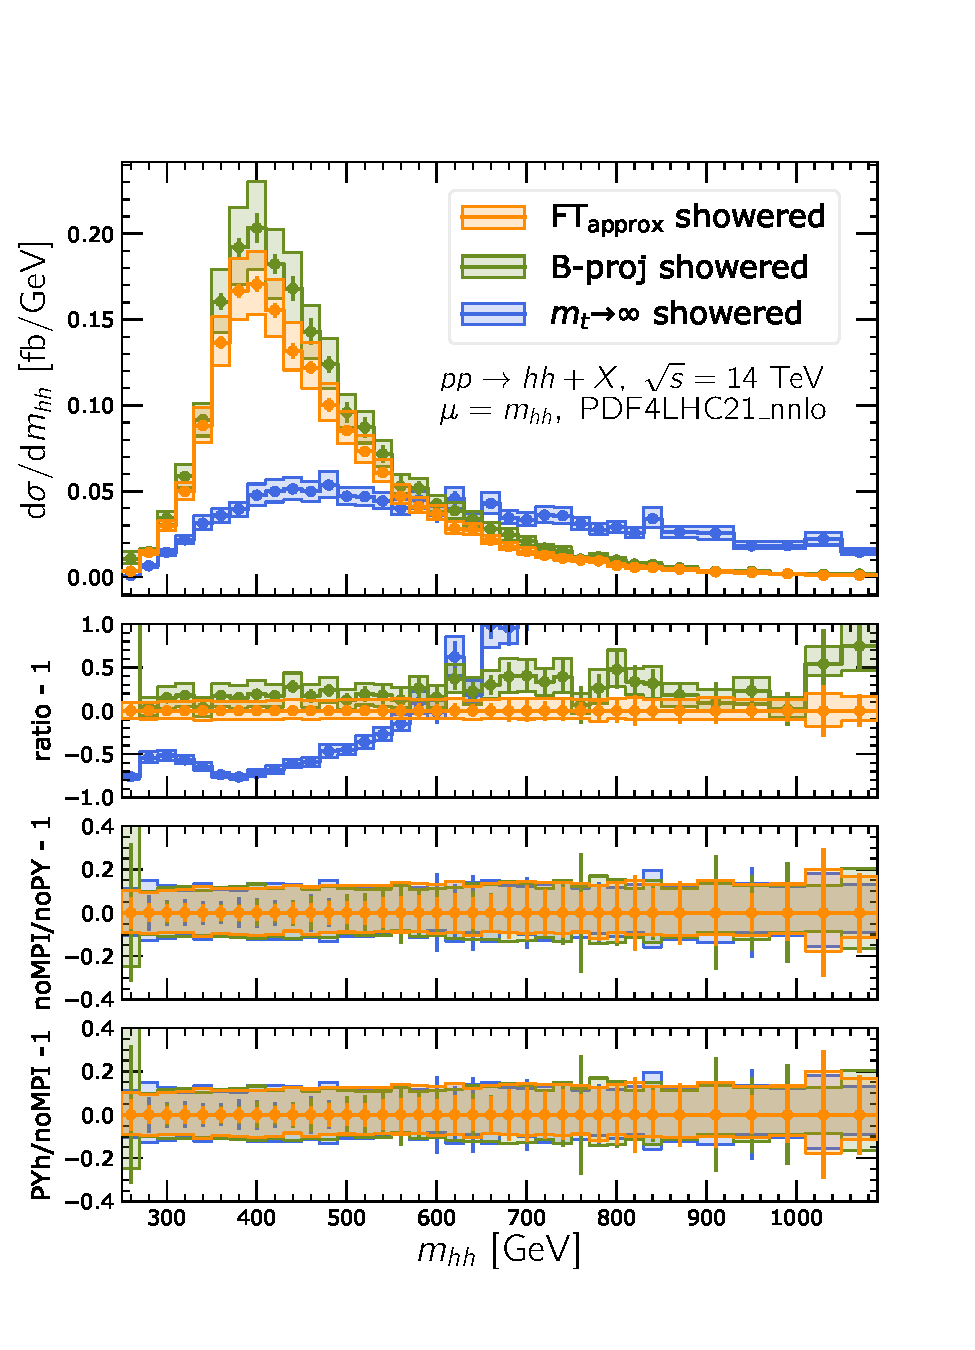
\includegraphics[width=0.49\textwidth]{NNLO_QCD_SM/NNLOgeneva/Images/Higgs_Pair_mass14-tev-showered_hhlabels.pdf} \hfill
  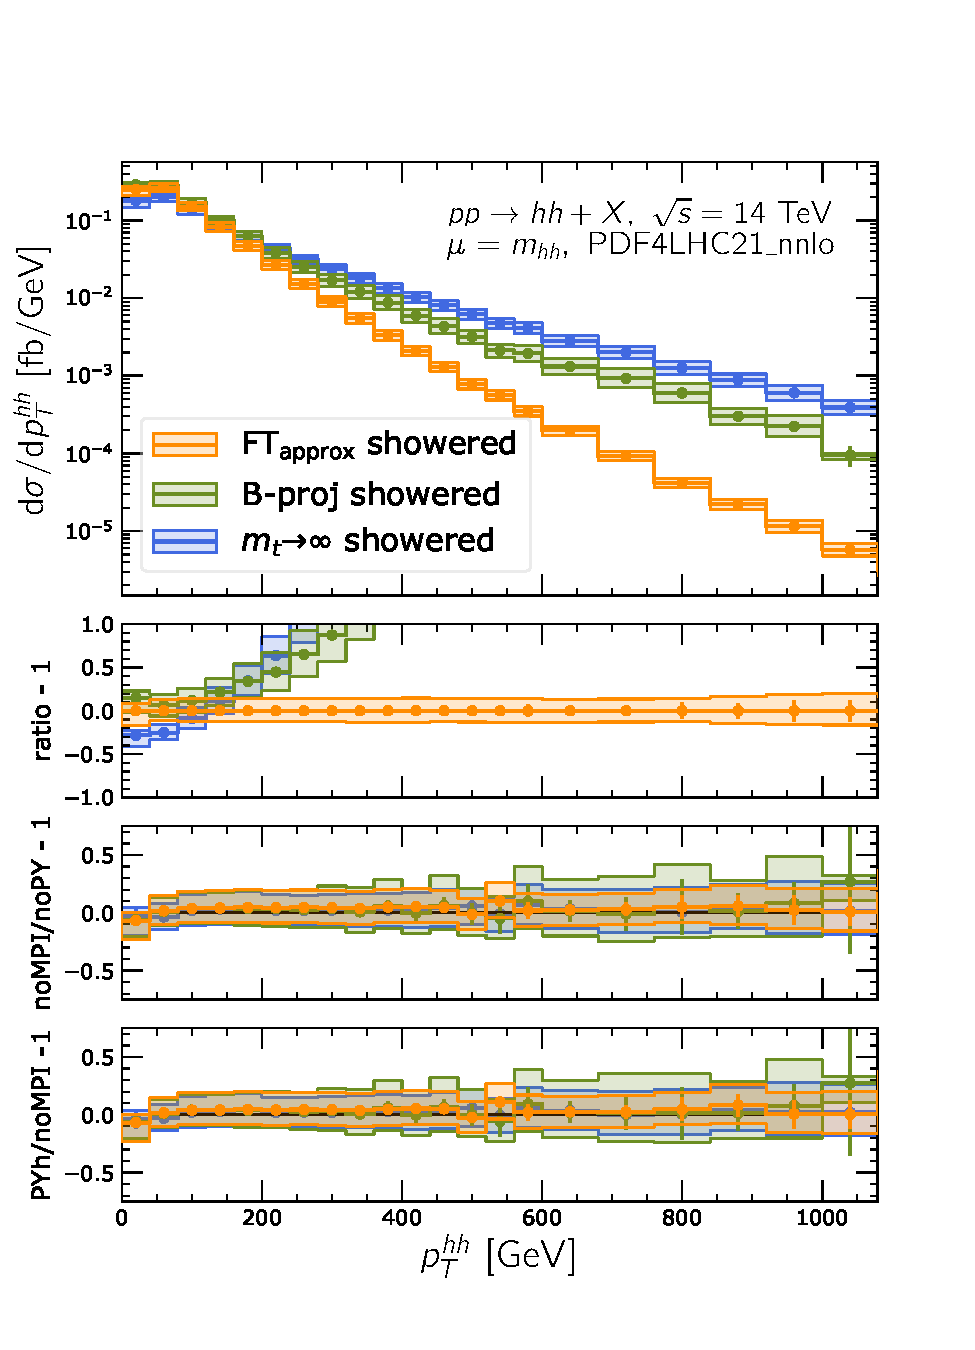
\includegraphics[width=0.49\textwidth]{NNLO_QCD_SM/NNLOgeneva/Images/Higgs_Pair_pT14-tev-showered_hhlabels.pdf}
  \caption{\label{fig:genevaplots}Comparison of showered predictions obtained with the three top quark mass approximations: $m_t \to \infty$
  (blue), B-proj (light green) and \ftapprox (dark orange), shown for various differential distributions.
  These include the invariant mass of the Higgs boson pair ($m_{hh}$)
  and the transverse momentum of the pair system ($p_T^{hh}$).
  Results are obtained at $\sqrt{s} = 14$ TeV, with central scale $\mu = m_{hh}$,
  using the \texttt{PDF4LHC21\_nnlo} PDF set and 3-point scale variations.
  Results shown are from Ref.~\cite{Alioli:2025xcu}.
}
\end{center}
\end{figure}


The inclusion of finite top quark mass effects leads to a significant impact,
much larger than that of the parton shower itself.
For the Higgs boson pair invariant mass this is a consequence of the shower unitarity
with respect to fully inclusive observables and thus follows by construction.
For the transverse momentum of the pair of Higgs bosons, the shower
induces a small effect in the first few bins, of approximately $5\%$ relative to the
partonic predictions.
Finally, by comparing the last two ratio panels, we can observe that the hadronization and MPI
effects are marginal and affect all mass approximations in the same way.
